\documentclass[
	%a4paper, % Use A4 paper size
	letterpaper, % Use US letter paper size
]{jdf}

\usepackage{multicol}

\addbibresource{references.bib}

\author{Steven Billington}
\email{sbillington3@gatech.edu}
\title{Homework \#2}

\begin{document}
%\lsstyle

\maketitle

%\begin{abstract}
%	Welcome to Joyner Document Format (JDF) v2.2! JDF is primarily intended to standardize page lengths while ensuring readability. Note that you are required to use JDF for all written assignments, but we will not perform explicit formatting checks. So, while improper formatting may be subject to penalties, you should not worry too much about whether your submission conforms to every minute detail; the most important elements are margins, font, font sizes, and line spacing. Just make a copy of one of the provided templates and replace its contents with your own, using the built-in paragraph styles.\footnote{Here are instructions for \href{https://support.office.com/en-us/article/Video-Using-Styles-in-Word-9db4c0f4-2754-4294-9758-c14a0abd8cfa}{Microsoft Word}, \href{https://support.apple.com/guide/pages/intro-to-paragraph-styles-tanaa39b0aa3/mac}{Apple Pages}, and \href{https://www.bazroberts.com/2016/04/19/google-docs-paragraph-styles-headings/}{Google Docs}.} If you do so, you do not need to verify that the style was followed.
%\end{abstract}

\section{Question \#1 - What is a Sandwich?}
\subsection{Billington Based Classification}
What is a sandwich? Is a hotdog a sandwich? I have been given a list of dishes and need to decide whether or not they are sandwiches. This will assist in helping me classify whether a hotdog is a sandwich.
\begin{multicols}{2}
\small
\begin{itemize}
    \item BLT on white bread. Sandwich.
    \item Hamburger. Sandwich
    \item Turkey and Swiss on a Potato roll. Sandwich.
    \item Meatball sub. Sandwich.
    \item Tuna Salad on brioche. Sandwich.
    \item Chicken Wrap. Not a Sandwich.
    \item Chip Butty. Sandwich.
    \item Burrito. Not a Sandwich.
    \item Ice Cream Sandwich. Not a Sandwich
    \item Grilled Cheese. Not a Sandwich.
    \item Turkey Hero. Sandwich.
    \item Ice Cream Taco. Not a Sandwich.
    \item Vada Pav. Not a Sandwich.
    \item Toast. Not a Sandwich.
    \item Cheese Quesadilla. Not a Sandwich.
    \item Toaster Strudel. Not a Sandwich.
    \item Veggie Burger. Sandwich.
    \item Klondike Bar. Not a Sandwich.
    \item Egg \& Cheese Biscuit. Not a Sandwich.
    \item Buttered Biscuit. Not a Sandwich.
    \item Gyro. Not a Sandwich.
    \item Sushi rolls. Not a Sandwich.
    \item Patty Melt. Sandwich.
    \item Calzone. Not a Sandwich.
    \item Sloppy Joe. Sandwich.
\end{itemize}
\end{multicols}
%Prior to beginning this question, consider one of the great internet debates of our time: what is a sandwich? First, take the following list of dishes and decide whether each one is a sandwich. In your assignment, start with a list of which of these you consider sandwiches, and which you do not. If you are unfamiliar with any of these types of sandwich, you should be able to Google them and find out what they are.
%BLT on white bread; hamburger; turkey and swiss on potato roll; meatball sub; tuna salad on brioche; chicken wrap; chip butty; burrito; ice cream sandwich; grilled cheese; turkey hero; ice cream taco; vada pav; toast; cheese quesadilla; toaster strudel; veggie burger; Klondike bar; egg \& cheese biscuit; buttered biscuit; gyro; sushi rolls; patty melt; calzone; sloppy joe.
\subsection{Incremental Concept Learning}
The potential series of sandwiches that I will use to demonstrate Incremental Concept Learning are "BLT on White Bread", "Patty Melt", "Ice Cream Sandwich", and "Chicken Wrap". Starting with the initial sandwich on that list of four, I created the following rudimentary diagram (Figure 1) describing a rudimentary concept of a sandwich. It is a bread object supporting a filling or middle layer of vegetables and meats which then supports another bread object. From there, we move to Patty Melt. A Patty Melt includes the middle layer of meat, but may not require vegetables. Also a Patty Melt typically includes cheese of some sort as a part of the middle layer. We will generalize from the initial diagram in Figure 1 to a more inclusive definition seen in Figure 2 where the middle layer becomes "Not Bread" (Close-interval heuristic to include everything but bread). But what about Ice Cream Sandwiches? I did not consider them sandwiches so some additional logic is missing here. 

\begin{figure}[h]
	\centering
	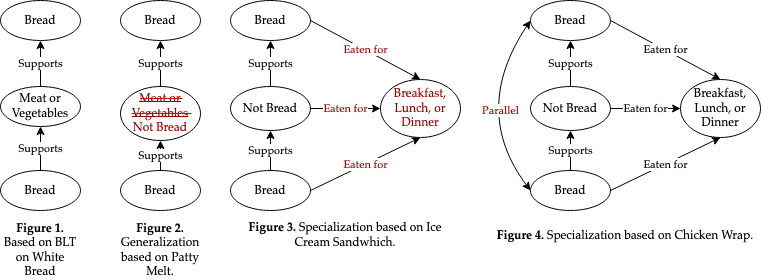
\includegraphics{SandwichFiguresCorrection.jpg}
	\label{fig:flowchart}
\end{figure}

From Figure 2 to Figure 3 I add a different node, a "meal" node is included where the meal is breakfast, lunch, or dinner. This specialization will exclude ice cream sandwiches since an ice cream sandwich is not a meal for breakfast, lunch or dinner. Finally we move to the Chicken Wrap, which is not a Sandwich. From here we will include a new relationship (Figure 4) between the two nodes of Bread that state that the flat portions of the bread to be parallel from one another. This specialization, a require link heuristic, would eliminate any configurations of wraps where a wrap is definitely not parallel from itself or any other wrap around it since it they touch.

Is there any sandwich type that will break the mold from the long list above? A Grilled Cheese would violate the current model since it meets all standards described but is not a sandwich and require additional specialization in order to eliminate as an option.
%Once you’ve labeled each of those, illustrate the process of incremental concept learning using a series of potential sandwiches. Construct a model of what a sandwich is, noting which heuristics are used to specialize and generalize the model with each additional positive or negative example. Step through the process with at least four potential sandwiches, at least two positive and two negative examples. Then, briefly note whether any of the sandwiches you did not include would make a significant difference to the model if you had chosen to go that far.
\subsection{Classification}
The rules I created to help classify a sandwich are:
\begin{enumerate}
    \item Has Sliced Bread?
    \item Is Savory?
    \item Has at least one distinct filling layer?
\end{enumerate}

Based on these three rules the following 6 items from the list above fall into the not-sandwich or sandwich camp based on the classification rules.

\begin{table}[h]
    \small
    \centering
    \caption{Sandwich classification according to three rules. Matches original means matches the classification according to Billington (1.1.)}
    \begin{tabular}{l|l|l|p{2 cm}|l|p{1.75 cm}}
        \textbf{Name} & \textbf{Sliced Bread?} & \textbf{Savory?} & \textbf{Has at least 1 distinct filling layer?} & \textbf{Is Sandwich?} & \textbf{Matches original?}\\
        \toprule[0.5pt]
        Hamburger & Yes & Yes & Yes & Yes & Yes\\
        Turkey Hero & Yes & Yes & Yes & Yes & Yes\\
        Meatball Sandwich & Yes & Yes & Yes & Yes & Yes\\
        Ice Cream Taco & No & No & Yes & No & Yes\\
        Toaster Strudel & No & No & Yes & No & Yes\\
        Egg \& Cheese Biscuit & Yes & Yes & Yes & Yes & No\\
    \end{tabular}
    \label{tab:my_label}
\end{table}

Based on the six sandwiches selected there needs to be some modification to the classification system that I constructed. First, the "Has at least one distinct filling layer" was met by each of the 6 selected food types. It was therefore not helpful in terms of helping to distinguish between sandwich and not sandwich. Finally, my rules were unable to correctly classify an egg \& cheese biscuit as "Not a Sandwich".

%Next, attempt a classification approach to defining a sandwich. Select a number of parameters (similar to “Lays eggs?” and “Has wings?” from the bird example in the Classification lecture) that would be useful in differentiating sandwiches. We recommend considering both structure and ingredients. Then, define values for those parameters for at least six sandwiches, and then construct an abstracted classification of what a sandwich is based on those values.
\subsection{Case-Based Reasoning}
For case-based reasoning I need to find which "sandwich" is most similar in nature to a hot dog. In this case the most similar is the Meatball Sandwich. Both include a long piece of bread that is baguette like in nature. The bread can be either completely bisected width wise, or cut through with width wise but still one piece of bread. In both cases the filling is a ground and shaped pieces of meat that can have a savory sauce covering the meat.
%Finally, answer the age old question, “Is a hot dog a sandwich?”, using each of three perspectives: the model you developed through incremental concept learning; the classifier you developed based on those parameters and their values; and a case-based reasoning approach. With regard to case-based reasoning, you need only comment on what sandwich you think would be drawn as most “similar” to a hot dog.
\subsection{Conclusion}
So is a hot dog a sandwich? 

Using the incremental learning concept it is not a sandwich. If the hot dog does not have the bread completely bisected width wise, which a hot dog bun most times does not, then it will fail to meet the "Parallel" relationship requirement between the two pieces of bread.

According to the classification rules constructed a hot dog is a sandwich since it a) Has sliced Bread, b) Is savory, c) has at least 1 distinct filling layer.

Finally, according to case based-reasoning the meatball sub is the closest match to a hot dog. Based on how similar they are, the only real difference is size and shape of the meat. A hot dog would be a sandwich according to case based reasoning.
\section{Question \#2 - Maria kicked the Can}
%Consider the sentence: “Maria didn’t say I kicked the can.”
\subsection{Frame Representation}
I have been tasked to take the sentence "Maria didn't say I kicked the can." and provide a frame representation for the sentence that an AI might be able to construct. See Figure 5 below for the frame representation constructed. An AI agent could start with determining which words in the sentence are action verbs, and then create frames around said verbs. From there the subject, direct object, and indirect object (if applicable) can be identified. Based on the type of noun the direct or indirect object is, we can establish sub-frames such as Person, Place, or Thing each with a differing set of slots or default-fillers. 
\setcounter{figure}{4}
\begin{figure}[h]
	\centering
	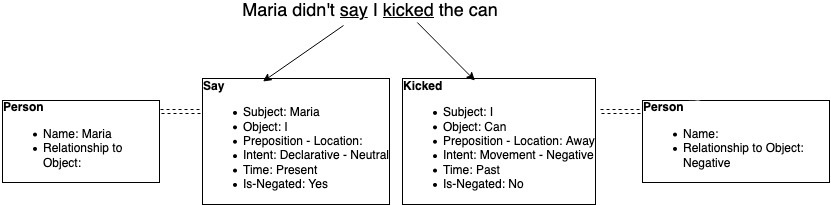
\includegraphics[height=6cm]{Original Maria.jpg}
	\caption{Frame representation of the sentence "Maria didn't say I kicked the can." Frames originally built around verbs.}
	\label{fig:flowchart}
\end{figure}
%First, explain how an AI agent might use the principles of Understanding to make sense of that sentence. As part of this, provide a frame representation of this sentence.
\subsection{Emphasis Changing Frame Representation}
If the sentence had different emphasis placed on it, such as "\textbf{Maria} didn't..." or "...say I \textbf{kicked}...", how could our frames change value? For the first example with the emphasis being on Maria (see Figure 6 below), the primary noun or the noun in the subject case, then the frame will actually remove Maria as the subject for "say" since the word "didn't" negates Maria's place as the primary subject. In this case the frame for say will have an empty Subject, the is-negated slot flips to "No" because someone or something did say that "I kicked the can", and the sub frame of person will change from a filled name slot to an empty slot.
\begin{figure}[h]
	\centering
	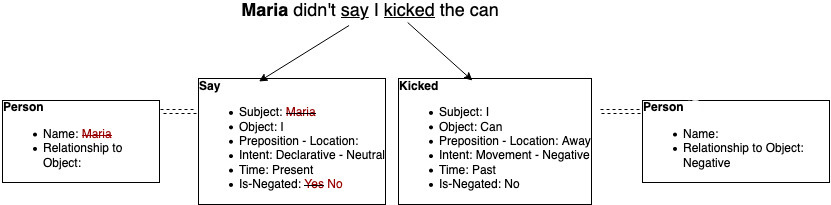
\includegraphics[height=6cm]{Emphasis Maria.jpg}
	\caption{Emphasis on "Maria" places negates Maria being the subject for the Say frame.}
	\label{fig:flowchart}
\end{figure}

\begin{figure}[h]
	\centering
	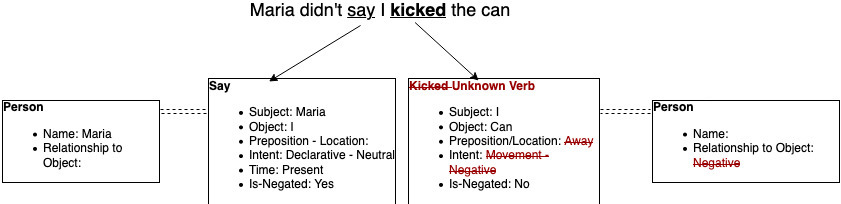
\includegraphics[height=6cm]{Emphasis Kicked.jpg}
	\caption{Emphasis on "kicked" negates the entire "kick" frame into an unknown verb frame.}
	\label{fig:flowchart}
\end{figure}

When the emphasis is instead on "kicked" then there is question for what the verb / action between the direct object (I) and the indirect object (the can) in the sentence. As for how this changes the frame, it negates the Kicked frame entirely into an unknown verb. At that point we can still make assumptions about subject, and object (and therefore the subframes can still hold true for the nouns such as the Person frame in Figure 7 for I). However, an AI agent would then be unable to determined the values for the Preposition/Location slot since those can only be filled in based on default fillers implied by the verb or by direct prepositions in the sentence, as well as the intent slot since that also receives a default-filler based on the action verb used.
%Second, imagine that the sentence had a different emphasis placed on it. “Maria didn’t say I kicked the can”, for example, implies that while someone said I kicked the can, Maria wasn’t the one who said that. “Maria didn’t say I kicked the can” implies while Maria said I did something to the can, she didn’t say I kicked it. Emphasizing any individual word changes the implication of the sentence.

%Explore how the AI agent might be able to understand how different emphases alter the meaning of the sentence. What additional knowledge or abilities would it need to have? As part of this, provide a frame representation that captures these new understandings. You must provide frame representations for at least two different interpretations of the sentence, but you may provide more.
\subsection{Literal or Figurative}
But what of the idiom "kicked the can"? It could mean to put off work or an action until a later time, or it could mean perishing, or it could be a literal kicking of a can. How would an AI agent be able to distinguish between the literal and figurative meaning behind the term? An AI agent may use Thematic Role Systems to create multiple types of frames based on common literal and figurative forms for the verb, which in this case would be kicked. From there individual slots would attempt to be filled for the AI agent across all of the frames and the frame that has most of the slots filled would be the frame that would be used.
%Finally, discuss how an AI agent might be able to infer whether this sentence is to be taken literally or figuratively. How would an AI agent decide whether the statement describes a literal can or the figurative idea of putting work off for a later date?
\section{Question \#3 - Toronto Declaration}
The Toronto Declaration was established in 2018 as a guiding document for protecting individual rights and preventing discrimination within machine learning and AI systems \citep{Toronto}. The major sections of the document are summarized below.
\subsection{Summary}
%The Preamble...
The "Preamble" for the Toronto Declaration lays the groundwork for why a Declaration needs to be established in the first place. Machine Learning systems, without proper forethought, monitoring, and auditing can exacerbate issues of equality and discrimination \citep{Toronto}.

%Using the Framework...
The "Using the Framework" section of the Toronto Declaration begins with establishing what the scope for the human right to equality and non-discrimination entails "... such as race, colour, sex, language, religion, political or other opinion, national or social origin, property, birth or other status" \citep{Toronto}.

%Duties of States...
The "Duties of States", according to the Declaration, include responsibilities around the state use of machine learning systems that include identifying risks, ensuring transparency and accountability, and enforcing oversight. The state must also promote diversity, and hold private entities accountable \citep{Toronto}.

%Responsibilities of Private Sector Actors...
The "Responsibilities of Private Sector Actors" include the process of exercising the "human rights due diligence" process that includes i) identifying potential discriminatory outcomes, ii) taking action to prevent and mitigate discrimination, and iii) submit high-risk systems for potential equality and discrimination abuses for third-party audits \citep{Toronto}.

%Right to an Effective Remedy...
Finally, the "Right to an Effective Remedy", posits that states and private entities must have a system in place to allow for transparency and within machine learning systems as well as accountability for violations \citep{Toronto}.
% Research the Toronto Declaration. Summarize each of its top-level sections (the Preamble, Using the Framework…, Duties of States, Responsibilities of Private Sector Actors, and Right to an Effective Remedy).
\subsection{Trade-Offs}
There are definite advantages to widespread adoption of the Toronto Declaration. If the declaration were completely disregarded then there will be machine learning systems that either incidentally or purposefully violate equality and non-discrimination rights. For an example of incidental violation of equality and non-discrimination, the ProPublica article "Machine Bias" lists many real life examples of how an algorithm that is used in the justice system not only provides recommended "risk assessments" that not only have a poor correlation with the likelihood of a crime to occur, but also disproportionately target African Americans \citep{Machine_Bias}. There are definite risks to citizens if the declaration is discarded. It could include a loss of opportunity. An AI system that helps match individuals to potential job openings may not provide an individual with all possible job openings if there is unseen prejudice and bias. There could be financial loss. An individual may not be recommended a loan with more favorable rates based on a system that includes prejudice and bias.

%Steven, you need your sources here. Don't forget propublica... https://www.propublica.org/article/machine-bias-risk-assessments-in-criminal-sentencing 

But what are potential disadvantages to adopting the entirety of the Toronto Declaration? Most private companies of small to medium size will argue that there is an economic cost to implementing systems of audits, having continuous oversight, and the training involved for individuals. There is also a risk that any system that would be implemented as a set of laws instead of completely opted in would be seen as even more government regulatory oversight and be opposed instead of embraced. The Toronto Declaration should be seen as a necessary good for society instead of a regulatory hurdle to sidestep since it will come at a cost. 
% Second, analyze the trade-offs inherent to the declaration. In following the declaration, what innovations or opportunities may be lost? If the declaration were discarded, what risks would there be to citizens?
\subsection{Opinion}
I believe that the Toronoto Declaration is a necessary and positive step towards universal equality and should be adopted by state and private entities alike. I agree that there needs to be state and private entity involvement to mitigate a lack of buy-in on both sides. I am strongly in favor of placing additional scrutiny into any machine learning or artificial intelligence system that has a role in judicial decision-making. I do not believe that there are portions of the Declaration that I disagree with, but I believe there are portions missing to make this document effective. There is no information about how states will keep one another accountable. The Declaration also does not provide any "strategy" for how any of this will be achieved. There is no suggested timeline, no way forward, and no recommendations.
% Third, determine your stance on the Toronto Declaration. What do you agree with? What do you disagree with? What would you remove, what would you keep, and what would you add?
\section{Question \#4 - AI and Human Augmentation}
The homework prompt for question 4 had us consider a thought experiment with Ethan, Sofia, and Akhila. Through various circumstances Ethan has become completely robotic, except for his biological brain. Sofia, on the other hand, is completely biological except for her brain. Finally, Akhila has no remaining organic portions to her. I assume that all three retain the same memories and personalities and have no discernible differences. 
% One role that futurists predict robotics and artificial intelligence will play in the future is human augmentation. Human physical abilities may be augmented with exoskeletons or robotic implements, and human cognitive abilities may be augmented with cybernetic implants. Some futurists suggest that parts of our bodies and brains could be replaced with technological improvements.

% Consider a thought experiment. There are three individuals in the future: Ethan, Sofia, and Akhila.

% Ethan, a mountain climbing enthusiast specializing in conquering the highest peaks in the solar system, decides to wholly embrace the physical augmentations available at the time. First, he opts to have his legs replaced by state-of-the-art robotic legs that never tire and can run several times faster than a typical person. Then, he replaces his arms with the industry standard reconfigurable extremities, which allow him to replace his hands with other tools at will. He then is a subject in a late-stage device development for a system that replaces his digestive and respiratory systems with technological alternatives for more convenient energy storage and distribution. Finally, after an accident that irreparably damages the bones in his jaw, he replaces his own face and head with a robotic container. In the end, the only organic part of Ethan remaining is his brain, housed in an otherwise robotic body.

% Sofia, on the other hand, does not opt for any bodily reconfiguration. However, as pilot of commuter starships, the demands on her attention span and working memory are extremely high. She thus undergoes a procedure that augments her frontal lobe. Several years later, new research reveals that the augmentation results in the brain increasingly relying on the implant, and thus ultimately she must have her frontal lobe and temporal lobe replaced by equivalent technological analogues. Later, to allow her to use a new generation of cybernetically-connected ship controls, she has her parietal and occipital lobes replaced; her original lobes are scanned to ensure its content is preserved in their new replacements, which also allow for direct API connections. In the end, Sofia’s entire brain has been replaced, though the content of her original brain was scanned and included in each replacement. Ethan and Sofia are opposites of one another; anything that Ethan had replaced, Sofia retained, and vice versa.

% Finally, Akhila, Ethan’s mountain climbing partner as well as Sofia’s regular copilot, ultimately undergoes all the same procedures as both of her friends, in roughly the same sequence. In the end, nothing organic is left from Akhila’s original body and brain.
\subsection{Identity Definition}
This scenario is remarkably similar to the short story / thought experiment "Where Am I" written by Daniel C. Dennett \citep{Dennett1978-DENWAI}. In the short story an individual was separated from their body but was able to wirelessly control their body. Which is the person and the sense of self? The body or the brain? Could one exist without the other? Similarly, if the aspect of personhood and identity is detached, such as with the "Ship of Theseus" thought experiment, would we consider a complete replacement of parts the same item? With all of these competing ideas and thoughts it is best to start with a clear definition of "Personhood" and "Identity" as it pertains to people in order to answer the thought experiment of Ethan, Sofia, and Akhila. 

Similar to the works of Francis J. Beckwith , I define "personhood" as an entity with the capacity to reach "human functionality" \citep{Beckwith}. In this case we would use human functionality through an extensional definition lens where we list all of the various functions that humans "could" do, such as the use of tools, thought, language, creative thought, use of music, warfare, etc., to define what human functionality entails.

Identity, on the other hand, I will define as the ability to self-identify and label all of the physical manifestations the physical realm that are controlled by a single cognitive system.

Under these conditions let us go over a few test instances to see where along the personhood and identity definitions the person, place, or thing lies. A car does not have personhood because it does not have the capacity for human actions, and it does not have identity since it does not have a cognitive system. A chimpanzee does not have personhood because it does not have the full capacity for human actions, but one can argue that they do have identity since they are able to recognize themselves through a mirror test \citep{Chimpanzee}. How about a baby? A baby has full personhood since they do have the potential for human actions, but do not have identity since they are unable to identify all of the physical portions of themselves that attribute to a singular cognitive system. With this in mind we return to Ethan, Sofia, and Akhila.
\subsection{Personhood and Identity for Ethan, Sofia, Akhila Thought Experiment}
Is Ethan still Ethan in spite of him replacing all of his physical parts. If we assume that if you maintain both personhood and identity then you are "the same", then yes Ethan is still the same. Ethan has the capacity for human actions if all of his parts are replaced by mechanical items as long as they are able to completely mimic human actions.Would Ethan still be Ethan if he had his entire body rebuilt at once? As long as the system still is completely able to maintain their potential for human actions, then yes Ethan still maintains his personhood. Ethan also still has a full sense of all of the parts that compose their cognitive system. Therefore Ethan is still the person Ethan. 

What of Sofia? Sofia has the potential to conduct human actions and therefore maintains her "personhood". If we assume that each item of Sofia's brain is physically within her body without any of the memory being offloaded into some type of "cloud" equivalent, then Sofia still maintains her identity. With both her personhood and identity intact, Sofia is still the person Sofia.

Finally, what of Akhila who has completely replaced a biological self with a completely inorganic one? Similar to Ethan the state of personhood is a question of whether the mechanical parts mimic human actions completely. If the parts still mimic human functions, then Akhila still maintains personhood. For identity, as long as Akhila still maintains a complete awareness of all the portions of their cognitive system, then they still maintain their identity. Ultimately Akhila is still Akhila. Would Akhila still be Akhila if a complete copy would be built after a tragic accident? I would argue that yes Akhila would maintain a sense of self with both personhood and identity. Continuity of both personhood and identity is not an additional criteria to maintain the self, only that the criteria for both personhood and identity are met.
% After all the procedures have been completed, who is still the same person they were originally? Is Ethan still Ethan? Is Sofia still Sofia? Is Akhila still Akhila? If any are not still the person they began as, at what point did they cease to be that person? Why?

% Provide your answers to the above questions, and argue for your perspective. In your argument, consider the significance of the narrative: would it be different if Ethan had his entire body replaced at once, or if an entire copy of Akhila was built from a backup after a tragic accident? Your argument should not be purely opinion-based; you should provide definitions for relevant concepts regarding personhood and identity, and construct your argument from those definitions.

\section{References}
\printbibliography[heading=none]
\end{document}